\documentclass[letterpaper,11pt]{article}
\oddsidemargin -1.0cm \textwidth 17.5cm

\usepackage[utf8]{inputenc}
\usepackage[activeacute,spanish, es-lcroman]{babel}
\decimalpoint
\usepackage{amsfonts,setspace}
\usepackage{amsmath}
\usepackage{amssymb, amsmath, amsthm}
\usepackage{comment}
\usepackage{float}
\usepackage{amssymb}
\usepackage{dsfont}
\usepackage{anysize}
\usepackage{multicol}
\usepackage{enumerate}
\usepackage{graphicx}
\usepackage[left=1.5cm,top=2cm,right=1.5cm, bottom=1.7cm]{geometry}
\setlength\headheight{1.5em} 
\usepackage{fancyhdr}
\usepackage{multicol}
\usepackage{hyperref}
\usepackage{wrapfig}
\usepackage{subcaption}
\usepackage{siunitx}
\usepackage{cancel}
\usepackage{mdwlist}
\pagestyle{fancy}
\fancyhf{}
\renewcommand{\labelenumi}{\normalsize\bfseries P\arabic{enumi}.}
\renewcommand{\labelenumii}{\normalsize\bfseries (\alph{enumii})}
\renewcommand{\labelenumiii}{\normalsize\bfseries \roman{enumiii})}


\begin{document}

\fancyhead[L]{\itshape{Facultad de Ciencias F\'isicas y Matem\'aticas}}
\fancyhead[R]{\itshape{Universidad de Chile}}

\begin{minipage}{11.5cm}
    \begin{flushleft}
        \hspace*{-0.6cm}\textbf{FI1000-6 Introducción a la Física Clásica}\\
        \hspace*{-0.6cm}\textbf{Profesora:} Paulina Lira\\
        \hspace*{-0.6cm}\textbf{Auxiliares:} Juan Cristóbal Castro \& Alejandro Silva\\
        \hspace*{-0.6cm}\textbf{Ayudantes:} Francisca Bórquez, Catalina Molina \& Erick Pérez\\
        
    \end{flushleft}
\end{minipage}

\begin{picture}(2,3)
    \put(366, 10){\includegraphics[scale=0.9]{2020-1/Imágenes/logo/dfi-fcfm.pdf}}
\end{picture}

\begin{center}
	\LARGE\textbf{Auxiliar \#6}\\
	\Large{Cuerdas y Poleas}
\end{center}

\vspace{-1cm}
\begin{enumerate}\setlength{\itemsep}{0.4cm}

\rfoot[]{pág. \thepage}

\item[]

\item Dos bloques unidos por una cuerda ideal, que pasa por una polea, descansan sobre planos lisos como se muestra en la Figura~\ref{fig:p1}. Si $M>m$ y $\alpha <\beta$, determine:
    \begin{enumerate}
        \item El sentido de movimiento del sistema
        
        \item La aceleración de los bloques
        
        \item Tensión de la cuerda
    \end{enumerate}

\item Considere el montaje mostrado en la Figura~\ref{fig:p2}. La masa $m_1$ es $n$ veces la masa $m_2$. Considerando poleas y cuerdas ideales, determine la aceleración de la masa $m_2$ a medida que $m_1$ desciende desde una altura $h$. ¿Cuál es la altura máxima del suelo a la que podrá subir $m_2$?

\item Considere dos masas $M$ y $m$ unidas por un hilo que pasa por una polea ideal tal como se muestra en la Figura~\ref{fig:p3}.
En cierto instante el hilo que sostenía a la masa $M$ se corta. Determine la aceleración de la masa $M$.
¿Qué pasa en los límites cuando $M>>m$ y $m>>M$?

\begin{figure}[h!]
    \centering
    \begin{subfigure}[t]{0.4\textwidth}
        \centering
        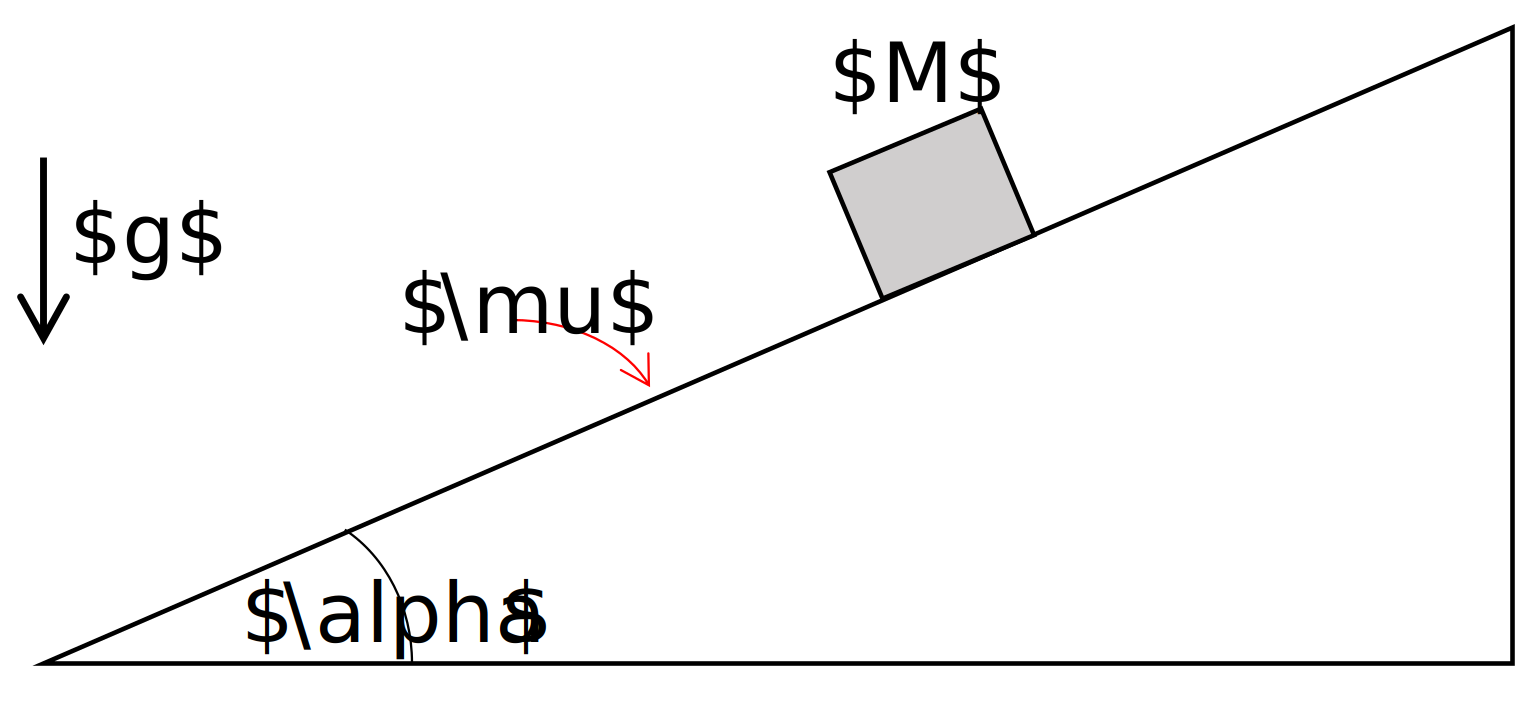
\includegraphics[width=0.8\linewidth]{2021-1/Imagenes/aux6/p1.pdf}
        \caption{P1}
        \label{fig:p1}
    \end{subfigure}
    \hspace{0.5em}
    \begin{subfigure}[t]{0.15\textwidth}
        \centering
        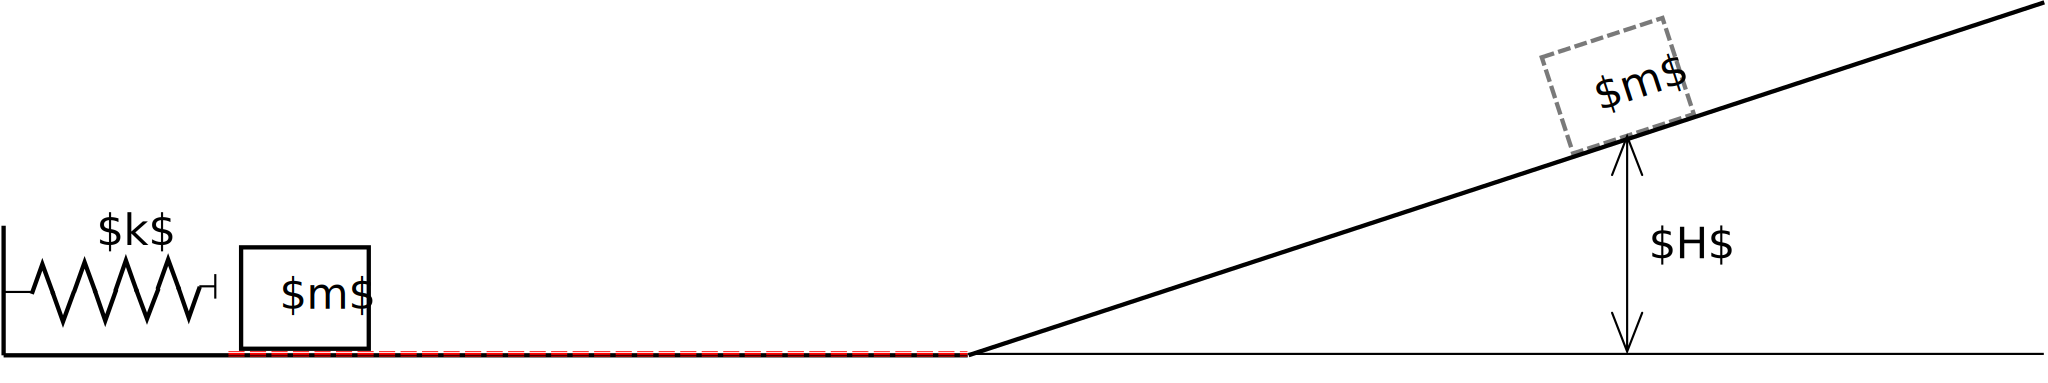
\includegraphics[width=0.85\linewidth]{2021-1/Imagenes/aux6/p2.pdf}
        \caption{P2}
        \label{fig:p2}
    \end{subfigure}
    \hspace{0.5em}
    \begin{subfigure}[t]{0.4\textwidth}
        \centering
        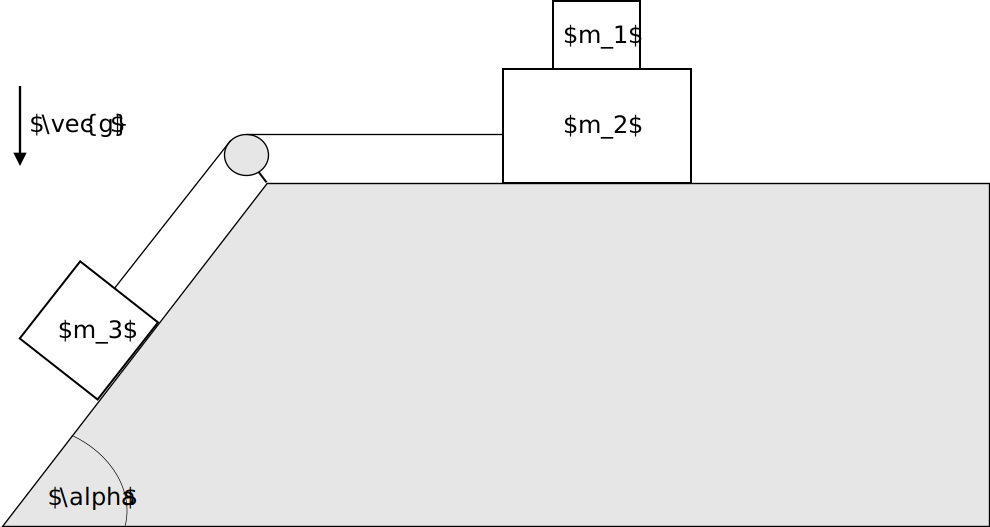
\includegraphics[width=0.4\linewidth]{2021-1/Imagenes/aux6/p3.pdf}
        \caption{P3}
        \label{fig:p3}
    \end{subfigure}
    \caption{}
\end{figure}


\end{enumerate}
\end{document}